% Options for packages loaded elsewhere
\PassOptionsToPackage{unicode}{hyperref}
\PassOptionsToPackage{hyphens}{url}
%
\documentclass[
]{book}
\usepackage{amsmath,amssymb}
\usepackage{lmodern}
\usepackage{iftex}
\ifPDFTeX
  \usepackage[T1]{fontenc}
  \usepackage[utf8]{inputenc}
  \usepackage{textcomp} % provide euro and other symbols
\else % if luatex or xetex
  \usepackage{unicode-math}
  \defaultfontfeatures{Scale=MatchLowercase}
  \defaultfontfeatures[\rmfamily]{Ligatures=TeX,Scale=1}
\fi
% Use upquote if available, for straight quotes in verbatim environments
\IfFileExists{upquote.sty}{\usepackage{upquote}}{}
\IfFileExists{microtype.sty}{% use microtype if available
  \usepackage[]{microtype}
  \UseMicrotypeSet[protrusion]{basicmath} % disable protrusion for tt fonts
}{}
\makeatletter
\@ifundefined{KOMAClassName}{% if non-KOMA class
  \IfFileExists{parskip.sty}{%
    \usepackage{parskip}
  }{% else
    \setlength{\parindent}{0pt}
    \setlength{\parskip}{6pt plus 2pt minus 1pt}}
}{% if KOMA class
  \KOMAoptions{parskip=half}}
\makeatother
\usepackage{xcolor}
\usepackage{color}
\usepackage{fancyvrb}
\newcommand{\VerbBar}{|}
\newcommand{\VERB}{\Verb[commandchars=\\\{\}]}
\DefineVerbatimEnvironment{Highlighting}{Verbatim}{commandchars=\\\{\}}
% Add ',fontsize=\small' for more characters per line
\usepackage{framed}
\definecolor{shadecolor}{RGB}{248,248,248}
\newenvironment{Shaded}{\begin{snugshade}}{\end{snugshade}}
\newcommand{\AlertTok}[1]{\textcolor[rgb]{0.94,0.16,0.16}{#1}}
\newcommand{\AnnotationTok}[1]{\textcolor[rgb]{0.56,0.35,0.01}{\textbf{\textit{#1}}}}
\newcommand{\AttributeTok}[1]{\textcolor[rgb]{0.77,0.63,0.00}{#1}}
\newcommand{\BaseNTok}[1]{\textcolor[rgb]{0.00,0.00,0.81}{#1}}
\newcommand{\BuiltInTok}[1]{#1}
\newcommand{\CharTok}[1]{\textcolor[rgb]{0.31,0.60,0.02}{#1}}
\newcommand{\CommentTok}[1]{\textcolor[rgb]{0.56,0.35,0.01}{\textit{#1}}}
\newcommand{\CommentVarTok}[1]{\textcolor[rgb]{0.56,0.35,0.01}{\textbf{\textit{#1}}}}
\newcommand{\ConstantTok}[1]{\textcolor[rgb]{0.00,0.00,0.00}{#1}}
\newcommand{\ControlFlowTok}[1]{\textcolor[rgb]{0.13,0.29,0.53}{\textbf{#1}}}
\newcommand{\DataTypeTok}[1]{\textcolor[rgb]{0.13,0.29,0.53}{#1}}
\newcommand{\DecValTok}[1]{\textcolor[rgb]{0.00,0.00,0.81}{#1}}
\newcommand{\DocumentationTok}[1]{\textcolor[rgb]{0.56,0.35,0.01}{\textbf{\textit{#1}}}}
\newcommand{\ErrorTok}[1]{\textcolor[rgb]{0.64,0.00,0.00}{\textbf{#1}}}
\newcommand{\ExtensionTok}[1]{#1}
\newcommand{\FloatTok}[1]{\textcolor[rgb]{0.00,0.00,0.81}{#1}}
\newcommand{\FunctionTok}[1]{\textcolor[rgb]{0.00,0.00,0.00}{#1}}
\newcommand{\ImportTok}[1]{#1}
\newcommand{\InformationTok}[1]{\textcolor[rgb]{0.56,0.35,0.01}{\textbf{\textit{#1}}}}
\newcommand{\KeywordTok}[1]{\textcolor[rgb]{0.13,0.29,0.53}{\textbf{#1}}}
\newcommand{\NormalTok}[1]{#1}
\newcommand{\OperatorTok}[1]{\textcolor[rgb]{0.81,0.36,0.00}{\textbf{#1}}}
\newcommand{\OtherTok}[1]{\textcolor[rgb]{0.56,0.35,0.01}{#1}}
\newcommand{\PreprocessorTok}[1]{\textcolor[rgb]{0.56,0.35,0.01}{\textit{#1}}}
\newcommand{\RegionMarkerTok}[1]{#1}
\newcommand{\SpecialCharTok}[1]{\textcolor[rgb]{0.00,0.00,0.00}{#1}}
\newcommand{\SpecialStringTok}[1]{\textcolor[rgb]{0.31,0.60,0.02}{#1}}
\newcommand{\StringTok}[1]{\textcolor[rgb]{0.31,0.60,0.02}{#1}}
\newcommand{\VariableTok}[1]{\textcolor[rgb]{0.00,0.00,0.00}{#1}}
\newcommand{\VerbatimStringTok}[1]{\textcolor[rgb]{0.31,0.60,0.02}{#1}}
\newcommand{\WarningTok}[1]{\textcolor[rgb]{0.56,0.35,0.01}{\textbf{\textit{#1}}}}
\usepackage{longtable,booktabs,array}
\usepackage{calc} % for calculating minipage widths
% Correct order of tables after \paragraph or \subparagraph
\usepackage{etoolbox}
\makeatletter
\patchcmd\longtable{\par}{\if@noskipsec\mbox{}\fi\par}{}{}
\makeatother
% Allow footnotes in longtable head/foot
\IfFileExists{footnotehyper.sty}{\usepackage{footnotehyper}}{\usepackage{footnote}}
\makesavenoteenv{longtable}
\usepackage{graphicx}
\makeatletter
\def\maxwidth{\ifdim\Gin@nat@width>\linewidth\linewidth\else\Gin@nat@width\fi}
\def\maxheight{\ifdim\Gin@nat@height>\textheight\textheight\else\Gin@nat@height\fi}
\makeatother
% Scale images if necessary, so that they will not overflow the page
% margins by default, and it is still possible to overwrite the defaults
% using explicit options in \includegraphics[width, height, ...]{}
\setkeys{Gin}{width=\maxwidth,height=\maxheight,keepaspectratio}
% Set default figure placement to htbp
\makeatletter
\def\fps@figure{htbp}
\makeatother
\setlength{\emergencystretch}{3em} % prevent overfull lines
\providecommand{\tightlist}{%
  \setlength{\itemsep}{0pt}\setlength{\parskip}{0pt}}
\setcounter{secnumdepth}{5}
\usepackage{booktabs}
\ifLuaTeX
  \usepackage{selnolig}  % disable illegal ligatures
\fi
\usepackage[]{natbib}
\bibliographystyle{apalike}
\IfFileExists{bookmark.sty}{\usepackage{bookmark}}{\usepackage{hyperref}}
\IfFileExists{xurl.sty}{\usepackage{xurl}}{} % add URL line breaks if available
\urlstyle{same} % disable monospaced font for URLs
\hypersetup{
  pdftitle={A Minimal Book Example},
  pdfauthor={John Doe},
  hidelinks,
  pdfcreator={LaTeX via pandoc}}

\title{A Minimal Book Example}
\author{John Doe}
\date{2023-05-18}

\usepackage{amsthm}
\newtheorem{theorem}{Theorem}[chapter]
\newtheorem{lemma}{Lemma}[chapter]
\newtheorem{corollary}{Corollary}[chapter]
\newtheorem{proposition}{Proposition}[chapter]
\newtheorem{conjecture}{Conjecture}[chapter]
\theoremstyle{definition}
\newtheorem{definition}{Definition}[chapter]
\theoremstyle{definition}
\newtheorem{example}{Example}[chapter]
\theoremstyle{definition}
\newtheorem{exercise}{Exercise}[chapter]
\theoremstyle{definition}
\newtheorem{hypothesis}{Hypothesis}[chapter]
\theoremstyle{remark}
\newtheorem*{remark}{Remark}
\newtheorem*{solution}{Solution}
\begin{document}
\maketitle

{
\setcounter{tocdepth}{1}
\tableofcontents
}
\hypertarget{about}{%
\chapter{About}\label{about}}

This is a \emph{sample} book written in \textbf{Markdown}. You can use anything that Pandoc's Markdown supports; for example, a math equation \(a^2 + b^2 = c^2\).

\hypertarget{usage}{%
\section{Usage}\label{usage}}

Each \textbf{bookdown} chapter is an .Rmd file, and each .Rmd file can contain one (and only one) chapter. A chapter \emph{must} start with a first-level heading: \texttt{\#\ A\ good\ chapter}, and can contain one (and only one) first-level heading.

Use second-level and higher headings within chapters like: \texttt{\#\#\ A\ short\ section} or \texttt{\#\#\#\ An\ even\ shorter\ section}.

The \texttt{index.Rmd} file is required, and is also your first book chapter. It will be the homepage when you render the book.

\hypertarget{render-book}{%
\section{Render book}\label{render-book}}

You can render the HTML version of this example book without changing anything:

\begin{enumerate}
\def\labelenumi{\arabic{enumi}.}
\item
  Find the \textbf{Build} pane in the RStudio IDE, and
\item
  Click on \textbf{Build Book}, then select your output format, or select ``All formats'' if you'd like to use multiple formats from the same book source files.
\end{enumerate}

Or build the book from the R console:

\begin{Shaded}
\begin{Highlighting}[]
\NormalTok{bookdown}\SpecialCharTok{::}\FunctionTok{render\_book}\NormalTok{()}
\end{Highlighting}
\end{Shaded}

To render this example to PDF as a \texttt{bookdown::pdf\_book}, you'll need to install XeLaTeX. You are recommended to install TinyTeX (which includes XeLaTeX): \url{https://yihui.org/tinytex/}.

\hypertarget{preview-book}{%
\section{Preview book}\label{preview-book}}

As you work, you may start a local server to live preview this HTML book. This preview will update as you edit the book when you save individual .Rmd files. You can start the server in a work session by using the RStudio add-in ``Preview book'', or from the R console:

\begin{Shaded}
\begin{Highlighting}[]
\NormalTok{bookdown}\SpecialCharTok{::}\FunctionTok{serve\_book}\NormalTok{()}
\end{Highlighting}
\end{Shaded}

\hypertarget{preface}{%
\chapter{Preface}\label{preface}}

This book is dedicated to my wife Balqisu.

To all the young scientists who would benefit from this book and colleagues who
through every small or big way helped me write this, I say a big thank you.
\citet{diener1996most}

The motivation for writing this book comes from the dire and urgent need for
many, especially those in developing countries to have and use a freely
available yet sophisticate statistical software. In regions where buying a
statistical software is often beyond the means of most persons R comes as a
great relief. There is a huge gap between theoretical and practical knowledge of
using statistical applications by many scientists. \textbf{R}, an open source
statistical software offers a unique but important opportunity to bridge this
gap.

The focus of this book is to introduce data analysis and R to persons with very
little knowledge in both. This step by step introduction to data analysis and R
is deliberately organised to have very limited text but lots of practical
examples. Readers are advised to replicate the examples as they read along, at
least to have a feel of how these work in R.

The book comes with a set of data in many file formats. Some are fictitious
while a few are real data modified for public use. The datasets are freely
available online at
\url{https://dl.dropboxusercontent.com/u/1673032/Intro_R_STI_Data_14_10_2014.rar}.

As this is essentially an introductory text, it is set up to sparingly use
packages1 other than the R base packages that comes with the default setup.
Occasionally however other packages are mentioned especially when it comes to
the graphics where the ``lattice'' and ``ggplot2'' packages are used. These are kept
to the minimum as new readers may find it confusing when they are constantly
being asked to download and install one package after the other.

As a general rule for this book, functions and their options are printed in
monospaced font with opening and closing brackets. Packages are written in
monospaced without brackets. Console output are written in monospaced font and
with a grey background. ''Urls'' and internet links are written in hypertext
format for easy access to these sites once a reader is connected to the internet.
Specific datasets are written in courier new font with a file extension such as
.csv, .txt etc.

\hypertarget{introduction}{%
\chapter{Introduction}\label{introduction}}

\hypertarget{the-statistical-data-analyst}{%
\section{The statistical data analyst}\label{the-statistical-data-analyst}}

Statistical data analysis is more than just using a computer software to
generate a set of results. It involves the basic understanding of the data type being analysed, the best way to analyse and then present such data to make sense to the population at large. Thus the data analyst :

\begin{enumerate}
\def\labelenumi{\arabic{enumi}.}
\tightlist
\item
  Must understand the genesis (study methodology) involved in obtaining the
  data in the first place. Conclusions from the same data may be different
  depending on the study methodology used and hypothesis being tested. It is very prudent therefore that the statistical data analyst be involved in the data collection process right from the beginning.
\item
  Should be able to point out errors in the data collection process in the very early stages to avoid wasting valuable resources on data that may not answer the question at hand.
\item
  Provide valuable advice on the best method of analysing the data at hand.
\item
  Perform the analysis in a scientifically sound manner applying the most
  current and statistically appropriate principles.
\item
  Be able to present the result of the analysis in a manner that makes it easy for literally all persons without statistical and analytical expertise to completely understand with the least effort. This requires the statistical data analyst to be in a position to explain the analysis in the ''layman's language''.
\item
  Finally the data analyst must know his limit. There are often instances where the analyst should seek ''professional'' help even though he/she may feel he/she is on the right path. It never hurts to seek a second opinion from your peers.
\end{enumerate}

It therefore goes without saying from the prior discussion that the data analyst
must have a firm understanding of statistical and research methodology.

\hypertarget{statistical-software}{%
\section{Statistical software}\label{statistical-software}}

Some years back, statistical analysis was one of the most tedious processes done mainly by dedicated statisticians. With the advent of computers and statistical software it has become rather handy with many advantages but some disadvantages as well.

The main advantages are:

\begin{enumerate}
\def\labelenumi{\arabic{enumi}.}
\tightlist
\item
  The tremendous speed with which large data is processed and results obtained.
\item
  The accuracy of the statistical calculations performed. Computers do not make mistakes but one has to beware of rounding in some software. Some software can perform calculations to specific number of decimal places. Therefore when one is
  confronted with a figure such as 1.00377655432 the software may work with
  1.0037765, leaving out the last four digits. Calculations using this truncated
  value is likely to have different result from the non-truncated figure, thus
  affecting the accuracy ofthe result.
\item
  Many modern statistical software have the ability to read data from varied
  sources and formats. This makes it easy to transfer data from one software to
  another without having to re-enter the data collected into the second computer
  or software.This transferability has enabled the use of other digital equipment such as smart phones, personal digital assistants and tablets for data collection. Data collected in this manner is said to be ready for cleaning and analysis, bypassing the data entry stage.
\item
  Plotting graphs is one of the most important uses of modern day computerised data analysis. Statistical software tend to make this rather tedious process almost hassle free and accords one the ability to redo the plot from scratch at the click of a button.
\end{enumerate}

Despite all these advantages many disadvantages are also inherent in the use of computers and statistical software. Some include:

\begin{enumerate}
\def\labelenumi{\arabic{enumi}.}
\tightlist
\item
  Many persons with very little or no statistical knowledge can manipulate data and come up with conclusions that often tend to be very spurious. The cliche ''Garbage In Garbage Out'' could not apply better than in this situation.
\item
  Many commonly used software tend to be very reliable and accurate. With the large number of often user written statistical software freely available online one needs to be cautious of the output generated. Some of these could actually be wrongly written codes producing faulty results.
\item
  Unfortunately the most used, reliable and accurate statistical software tend to be expensive as well. This not withstanding there are few, such as R that combines free and open source with versatility and reliability. This forms the basis for my choice of R for this book.
\end{enumerate}

\hypertarget{obtaining-and-installing-r}{%
\section{Obtaining and installing R}\label{obtaining-and-installing-r}}

R is a free software programming language and environment for data manipulation, calculation and graphical display. It can run on Windows, MacOS X and Unix systems. It has great applications in many academic fields including mathematics, economics and epidemiology. This capability has been enhanced by the many packages written by individuals over the years. R has a great advantage of being able to handle many datasets simultaneously. However this functionality comes at a cost which would be discussed in the subsequent chapters. R also has great graphics functionality but requires practice to harness full use of this.

Several advanced statistical and mathematical functionality such as regression
and survival analysis are also implemented in R.

R and its many packages are obtainable free from \url{http://cran.r-project.org/}.
The most current version as at writing this book is R-3.2.1-win32.exe. The
Windows version is installable on both the 32 and 64 bit operating systems.
Download the base file from \url{https://cran.r-project.org/bin/windows/base/}, save on your computer and install (preferably as an administrator) by double clicking the executable file and following the on-screen instructions.

\hypertarget{running-r}{%
\section{Running R}\label{running-r}}

After installation, two shortcuts similar to the figure below are placed on the desktop (windows version). On a Windows 8 64 bit machine both shortcuts for the 32 and 64 bit versions are placed on the desktop. Double click the desktop icon to launch R. A welcome screen as shown below is displayed in the console launched.

The \textgreater{} at the end of the output above is the command prompt and indicates R is
ready to be used. The R Console before you at this stage if running for the
first time will show a wide grey screen with a smaller white screen. The white
screen is the referred to as the console. We can type straight and obtain
requisite output on the console but I will strongly discourage this habit.

\hypertarget{r-as-a-calculator}{%
\section{R as a calculator}\label{r-as-a-calculator}}

The applicability of R in data analysis starts from its use as an overgrown
calculator. In this section we learn this simple task. Calculations in R can be
achieved simply by inputting and executing using the appropriate mathematical
operational symbols. These are

\(+\) addition\\
\(∗\) multiplication\\
\(−\) substraction\\
\(/\) division\\
\(∧\) raised to power or exponent

A couple of examples

\begin{Shaded}
\begin{Highlighting}[]
\DecValTok{7}\SpecialCharTok{+}\DecValTok{8}
\NormalTok{[}\DecValTok{1}\NormalTok{] }\DecValTok{15}

\NormalTok{(}\DecValTok{12{-}6}\NormalTok{)}\SpecialCharTok{/}\DecValTok{7}
\NormalTok{[}\DecValTok{1}\NormalTok{] }\FloatTok{0.8571429}
\end{Highlighting}
\end{Shaded}

\hypertarget{name-assignment-in-r}{%
\section{Name assignment in R}\label{name-assignment-in-r}}

All objects in R can be assigned names, values or attributes. This assignment
is achieved by using ``-\textgreater{}'' or ``\textless-''. The example below assigns the values 5 to
Kwame and 10 to Ama, their respective ages.

\begin{Shaded}
\begin{Highlighting}[]
\NormalTok{Kwame }\OtherTok{\textless{}{-}} \DecValTok{5}
\NormalTok{Ama }\OtherTok{\textless{}{-}} \DecValTok{10}
\end{Highlighting}
\end{Shaded}

Calling these names yield the values (ages) assigned. We can do that by typing
the names in the console.

\begin{Shaded}
\begin{Highlighting}[]
\NormalTok{Kwame}
\NormalTok{[}\DecValTok{1}\NormalTok{] }\DecValTok{5}
\NormalTok{Ama}
\NormalTok{[}\DecValTok{1}\NormalTok{] }\DecValTok{10}
\end{Highlighting}
\end{Shaded}

To add the ages of Kwame and Ama we can just do

\begin{Shaded}
\begin{Highlighting}[]
\NormalTok{Kwame }\SpecialCharTok{+}\NormalTok{ Ama}
\CommentTok{\#\textgreater{} [1] 15}
\end{Highlighting}
\end{Shaded}

\hypertarget{cross}{%
\chapter{Cross-references}\label{cross}}

Cross-references make it easier for your readers to find and link to elements in your book.

\hypertarget{chapters-and-sub-chapters}{%
\section{Chapters and sub-chapters}\label{chapters-and-sub-chapters}}

There are two steps to cross-reference any heading:

\begin{enumerate}
\def\labelenumi{\arabic{enumi}.}
\tightlist
\item
  Label the heading: \texttt{\#\ Hello\ world\ \{\#nice-label\}}.

  \begin{itemize}
  \tightlist
  \item
    Leave the label off if you like the automated heading generated based on your heading title: for example, \texttt{\#\ Hello\ world} = \texttt{\#\ Hello\ world\ \{\#hello-world\}}.
  \item
    To label an un-numbered heading, use: \texttt{\#\ Hello\ world\ \{-\#nice-label\}} or \texttt{\{\#\ Hello\ world\ .unnumbered\}}.
  \end{itemize}
\item
  Next, reference the labeled heading anywhere in the text using \texttt{\textbackslash{}@ref(nice-label)}; for example, please see Chapter \ref{cross}.

  \begin{itemize}
  \tightlist
  \item
    If you prefer text as the link instead of a numbered reference use: \protect\hyperlink{cross}{any text you want can go here}.
  \end{itemize}
\end{enumerate}

\hypertarget{captioned-figures-and-tables}{%
\section{Captioned figures and tables}\label{captioned-figures-and-tables}}

Figures and tables \emph{with captions} can also be cross-referenced from elsewhere in your book using \texttt{\textbackslash{}@ref(fig:chunk-label)} and \texttt{\textbackslash{}@ref(tab:chunk-label)}, respectively.

See Figure \ref{fig:nice-fig}.

\begin{Shaded}
\begin{Highlighting}[]
\FunctionTok{par}\NormalTok{(}\AttributeTok{mar =} \FunctionTok{c}\NormalTok{(}\DecValTok{4}\NormalTok{, }\DecValTok{4}\NormalTok{, .}\DecValTok{1}\NormalTok{, .}\DecValTok{1}\NormalTok{))}
\FunctionTok{plot}\NormalTok{(pressure, }\AttributeTok{type =} \StringTok{\textquotesingle{}b\textquotesingle{}}\NormalTok{, }\AttributeTok{pch =} \DecValTok{19}\NormalTok{)}
\end{Highlighting}
\end{Shaded}

\begin{figure}

{\centering 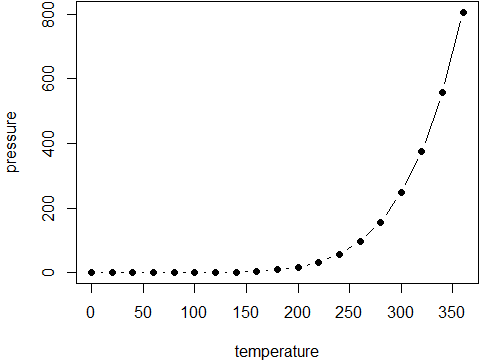
\includegraphics[width=0.8\linewidth]{52-cross-refs_files/figure-latex/nice-fig-1} 

}

\caption{Here is a nice figure!}\label{fig:nice-fig}
\end{figure}

Don't miss Table \ref{tab:nice-tab}.

\begin{Shaded}
\begin{Highlighting}[]
\NormalTok{knitr}\SpecialCharTok{::}\FunctionTok{kable}\NormalTok{(}
  \FunctionTok{head}\NormalTok{(pressure, }\DecValTok{10}\NormalTok{), }\AttributeTok{caption =} \StringTok{\textquotesingle{}Here is a nice table!\textquotesingle{}}\NormalTok{,}
  \AttributeTok{booktabs =} \ConstantTok{TRUE}
\NormalTok{)}
\end{Highlighting}
\end{Shaded}

\begin{table}

\caption{\label{tab:nice-tab}Here is a nice table!}
\centering
\begin{tabular}[t]{rr}
\toprule
temperature & pressure\\
\midrule
0 & 0.0002\\
20 & 0.0012\\
40 & 0.0060\\
60 & 0.0300\\
80 & 0.0900\\
\addlinespace
100 & 0.2700\\
120 & 0.7500\\
140 & 1.8500\\
160 & 4.2000\\
180 & 8.8000\\
\bottomrule
\end{tabular}
\end{table}

\hypertarget{parts}{%
\chapter{Parts}\label{parts}}

You can add parts to organize one or more book chapters together. Parts can be inserted at the top of an .Rmd file, before the first-level chapter heading in that same file.

Add a numbered part: \texttt{\#\ (PART)\ Act\ one\ \{-\}} (followed by \texttt{\#\ A\ chapter})

Add an unnumbered part: \texttt{\#\ (PART\textbackslash{}*)\ Act\ one\ \{-\}} (followed by \texttt{\#\ A\ chapter})

Add an appendix as a special kind of un-numbered part: \texttt{\#\ (APPENDIX)\ Other\ stuff\ \{-\}} (followed by \texttt{\#\ A\ chapter}). Chapters in an appendix are prepended with letters instead of numbers.

\hypertarget{footnotes-and-citations}{%
\chapter{Footnotes and citations}\label{footnotes-and-citations}}

\hypertarget{footnotes}{%
\section{Footnotes}\label{footnotes}}

Footnotes are put inside the square brackets after a caret \texttt{\^{}{[}{]}}. Like this one \footnote{This is a footnote.}.

\hypertarget{citations}{%
\section{Citations}\label{citations}}

Reference items in your bibliography file(s) using \texttt{@key}.

For example, we are using the \textbf{bookdown} package \citep{R-bookdown} (check out the last code chunk in index.Rmd to see how this citation key was added) in this sample book, which was built on top of R Markdown and \textbf{knitr} \citep{xie2015} (this citation was added manually in an external file book.bib).
Note that the \texttt{.bib} files need to be listed in the index.Rmd with the YAML \texttt{bibliography} key.

The \texttt{bs4\_book} theme makes footnotes appear inline when you click on them. In this example book, we added \texttt{csl:\ chicago-fullnote-bibliography.csl} to the \texttt{index.Rmd} YAML, and include the \texttt{.csl} file. To download a new style, we recommend: \url{https://www.zotero.org/styles/}

The RStudio Visual Markdown Editor can also make it easier to insert citations: \url{https://rstudio.github.io/visual-markdown-editing/\#/citations}

\hypertarget{blocks}{%
\chapter{Blocks}\label{blocks}}

\hypertarget{equations}{%
\section{Equations}\label{equations}}

Here is an equation.

\begin{equation} 
  f\left(k\right) = \binom{n}{k} p^k\left(1-p\right)^{n-k}
  \label{eq:binom}
\end{equation}

You may refer to using \texttt{\textbackslash{}@ref(eq:binom)}, like see Equation \eqref{eq:binom}.

\hypertarget{theorems-and-proofs}{%
\section{Theorems and proofs}\label{theorems-and-proofs}}

Labeled theorems can be referenced in text using \texttt{\textbackslash{}@ref(thm:tri)}, for example, check out this smart theorem \ref{thm:tri}.

\begin{theorem}
\protect\hypertarget{thm:tri}{}\label{thm:tri}For a right triangle, if \(c\) denotes the \emph{length} of the hypotenuse
and \(a\) and \(b\) denote the lengths of the \textbf{other} two sides, we have
\[a^2 + b^2 = c^2\]
\end{theorem}

Read more here \url{https://bookdown.org/yihui/bookdown/markdown-extensions-by-bookdown.html}.

\hypertarget{callout-blocks}{%
\section{Callout blocks}\label{callout-blocks}}

The \texttt{bs4\_book} theme also includes special callout blocks, like this \texttt{.rmdnote}.

You can use \textbf{markdown} inside a block.

\begin{Shaded}
\begin{Highlighting}[]
\FunctionTok{head}\NormalTok{(beaver1, }\AttributeTok{n =} \DecValTok{5}\NormalTok{)}
\CommentTok{\#\textgreater{}   day time  temp activ}
\CommentTok{\#\textgreater{} 1 346  840 36.33     0}
\CommentTok{\#\textgreater{} 2 346  850 36.34     0}
\CommentTok{\#\textgreater{} 3 346  900 36.35     0}
\CommentTok{\#\textgreater{} 4 346  910 36.42     0}
\CommentTok{\#\textgreater{} 5 346  920 36.55     0}
\end{Highlighting}
\end{Shaded}

It is up to the user to define the appearance of these blocks for LaTeX output.

You may also use: \texttt{.rmdcaution}, \texttt{.rmdimportant}, \texttt{.rmdtip}, or \texttt{.rmdwarning} as the block name.

The R Markdown Cookbook provides more help on how to use custom blocks to design your own callouts: \url{https://bookdown.org/yihui/rmarkdown-cookbook/custom-blocks.html}

\hypertarget{sharing-your-book}{%
\chapter{Sharing your book}\label{sharing-your-book}}

\hypertarget{publishing}{%
\section{Publishing}\label{publishing}}

HTML books can be published online, see: \url{https://bookdown.org/yihui/bookdown/publishing.html}

\hypertarget{pages}{%
\section{404 pages}\label{pages}}

By default, users will be directed to a 404 page if they try to access a webpage that cannot be found. If you'd like to customize your 404 page instead of using the default, you may add either a \texttt{\_404.Rmd} or \texttt{\_404.md} file to your project root and use code and/or Markdown syntax.

\hypertarget{metadata-for-sharing}{%
\section{Metadata for sharing}\label{metadata-for-sharing}}

Bookdown HTML books will provide HTML metadata for social sharing on platforms like Twitter, Facebook, and LinkedIn, using information you provide in the \texttt{index.Rmd} YAML. To setup, set the \texttt{url} for your book and the path to your \texttt{cover-image} file. Your book's \texttt{title} and \texttt{description} are also used.

This \texttt{bs4\_book} provides enhanced metadata for social sharing, so that each chapter shared will have a unique description, auto-generated based on the content.

Specify your book's source repository on GitHub as the \texttt{repo} in the \texttt{\_output.yml} file, which allows users to view each chapter's source file or suggest an edit. Read more about the features of this output format here:

\url{https://pkgs.rstudio.com/bookdown/reference/bs4_book.html}

Or use:

\begin{Shaded}
\begin{Highlighting}[]
\NormalTok{?bookdown}\SpecialCharTok{::}\NormalTok{bs4\_book}
\end{Highlighting}
\end{Shaded}


  \bibliography{book.bib,packages.bib}

\end{document}
